% Ubah kalimat sesuai dengan judul dari bab ini
\chapter{PROFIL PERUSAHAAN}
\vspace{4ex}

% Pengaturan ukuran indentasi
\setlength{\parindent}{7ex}

% Ubah konten-konten berikut sesuai dengan yang ingin diisi pada bab ini

\section{Sejarah PT. Aneka Tuna Indonesia}
\vspace{1ex}

PT. Aneka Tuna Indonesia berdiri pada didirikan pada bulan Oktober 1991, sebagai perusahaan gabungan antara Itochu 
Corporation dan Hagoromo Foods Corporation, yang merupakan pemilik merek tuna terkemuka di Jepang, serta satu 
perusahaan asing lainnya. 
\vspace{0.5ex}

Terletak di daerah pegunungan dengan panorama eksotis di Provinsi Jawa Timur Indonesia, kami mulai beroperasi secara 
komersial pada bulan November 1992, mengkhususkan diri dalam produksi dan penjualan tuna kalengan. 
\vspace{0.5ex}

Itochu melakukan penjualan dan manajemen keseluruhan, sementara Hagoromo Foods bertanggung jawab atas produksi. 
Semua mitra secara aktif terlibat dalam peningkatan kualitas produk termasuk pengiriman teknisi dari Jepang dan 
pengiriman teknisi lokal ke Jepang untuk pelatihan.
\vspace{0.5ex}

\section{Visi dan Misi}
\vspace{1ex}

PT. Aneka Tuna Indonesia memiliki visi dan misi sebagai berikut:
\vspace{0.5ex}

\begin{enumerate}[nolistsep]

  \item \textbf{Visi PT. Aneka Tuna Indonesia}
  \vspace{0.5ex}

  Menjadi produsen tuna kaleng terkemuka di dunia.
  \vspace{0.5ex}

  \item \textbf{Misi PT. Aneka Tuna Indonesia}
  \vspace{0.5ex}

  \begin{enumerate}[nolistsep]

    \item Menjadikan semua stakeholder bagian penting dari perusahaan.
    \vspace{0.5ex}

    \item Menghasilkan produk yang berkualitas, sehat dan aman, serta ramah lingkungan.
    \vspace{0.5ex}

  \end{enumerate}
  \vspace{0.5ex}

\end{enumerate}
\vspace{0.5ex}

\section{Struktur Organisasi}
\vspace{1ex}

Struktur Organisasi dari \lipsum[1]
\vspace{0.5ex}

% Contoh input gambar dengan format *.png
\begin{figure} [ht] \centering
  % Nama dari file gambar yang diinputkan
  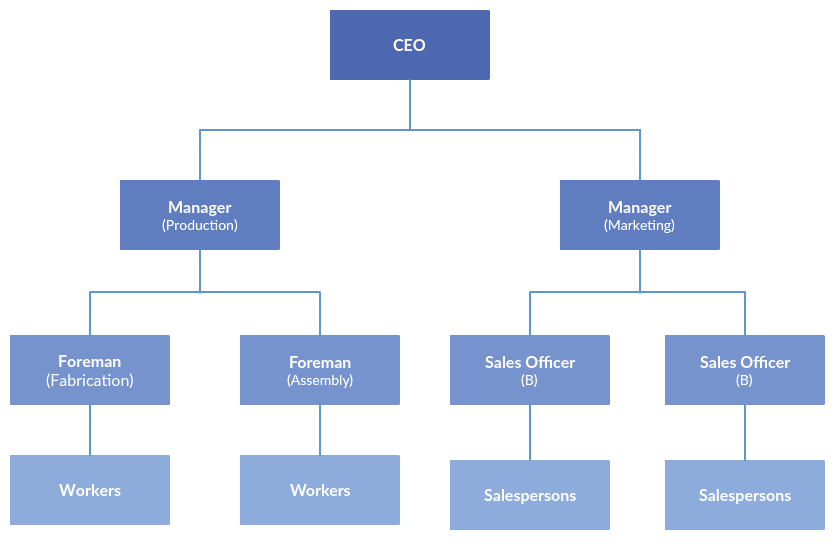
\includegraphics[scale=0.45]{gambar/struktur-organisasi.png}
  % Keterangan gambar yang diinputkan
  \caption{Struktur Organisasi PT. Aneka Tuna Indonesia}
  % Label referensi dari gambar yang diinputkan
	\label{fig:strukturOrganisasi}
\end{figure}

% Contoh penggunaan referensi dari gambar yang diinputkan
Seperti yang bisa dilihat pada \ref{fig:strukturOrganisasi}, \lipsum[1]
\vspace{0.5ex}
